\chapter{Software architecture}
The following sections present the software architecture of Modulo7.
\section{Server Side architecture}
\noindent Modulo7 is designed with the purpose of scalability. A block diagram of the components of the server side architecture is presented below :-
\begin{enumerate}
\item Source Converter : Converts music sources (e.g. music XML, midi etc) into modulo7's binary representation.
\item Music Theory Models : The model is a description of music theoretic criteria that can be applied on top of a song. Examples would be melodic contour, tonal histogram etc. 
\item Distributed Storage Mechanism : The modulo7 internal representation is a conversion to create a song representation with all the meta data of the song (Key, Scale,  etc) along with the sequences of note events stored as lists. This representation is then serialized and stored in and Hadoop Distributed File System. This allows for fault tolerance and a distributed deployment of the input data.
\item Lyrics Indexer : A distributed index of songs lyrics. This acts as a base on which standard techniques for similarity analysis might be applied. Alternatively it can provide a framework on which custom models (e.g. semantic intent of the song, correlation between music theory models and lyrics might also be applied).  
\item Lyrics similarity models : A set of similarity models that can be applied to an index. 
\item Query Engine : An SQL like interface to a client that allows you to gather and ascertain useful information (based on music theoretic criteria). 
\end{enumerate}

\begin{figure}
\centering
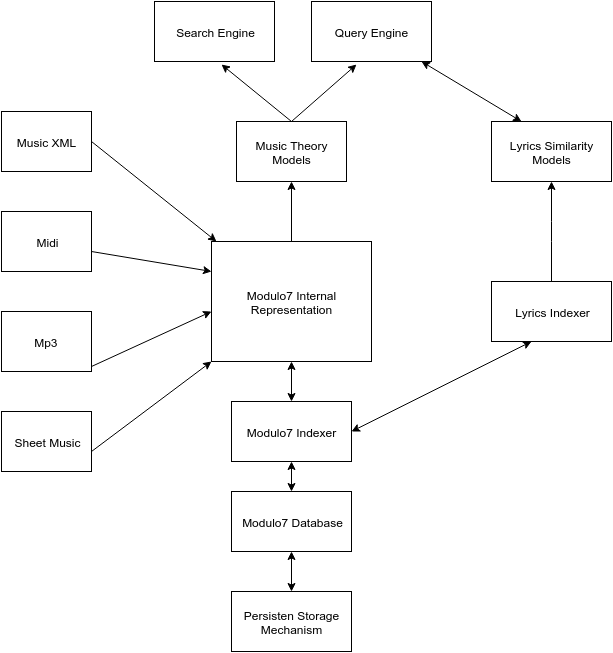
\includegraphics[width=\textwidth]{Modulo7Architecture.png}
\makeatletter
\let\@currsize\normalsize
\caption{Modulo7 architectural design}
\label{fig:figure}
\end{figure}
\newpage
\section{Client architecture}
The server exposes a sql like interface as well as a consumable API. Some sample queries would be :-
\begin{enumerate}
\item select midi files from database where $melodic\_complexity > some threshold$
\item select * from database where $artist = led\_zepplin \ and \ harmonic\_movement > harmonic\_movement(stairway\_to\_heaven)$
\item select $ num\_voices \ from \ Database \ where \ songName = someSong.midi$ 
\end{enumerate}

An API will also be exposed to the client along a remote invocation procedure. The API would primarily target single sources for specifics. Some example API would be :-
\begin{enumerate}
\item int getNumVoices(String midiFilePath)
\item double melodicContourMovement(String pngSheetFilePath)
\item double compareAverageAttack(String musicXMLFile)
\end{enumerate}

This API can be consumed for specific song analysis. As design this API will not work on a bulk of files like its sql counterpart. \\

Moreover the client also exposes a highly customized search engine based on the custom vector space representation of features extracted by Modulo7.

\section{Song sources}
\noindent At the heart of Modulo7's design is its song sources adaptors (or converters) into its own internal binary format. Each music source is a different representation and while certain sources ascribe what how music should be played (e.g musicxml, sheet music), other formats ascribe what is actually being played (e.g midi, mp3). There are many other music sources in existence (e.g guitar tablature, GUIDO format, humdrum format), but for the purposes of breadth and ubiquity, these four sources have been targeted as input for Modulo7. Note that acquiring features from each format is a domain specific challenge and inaccuracies are inherent because of that. The following subsections describe the individual formats in detail and the challenges encountered in parsing them.

\subsection{Midi format}
\noindent MIDI (short for Musical Instrument Digital Interface), is a technical specification for encoding of events on a midi enabled instrument and a protocol for interfacing and communicating between various midi enabled instruments. Typically any midi enabled electronic instrument when played, relays to its internal circuitry a message. Examples of such messages could be a particular note is being hit on a keyboard, a note is being hit off after being hit on, tempo based messages on the number of ticks per second etc. While MIDI is a technical specification for encoding music the score is being played, Modulo7 treats it as a symbolic representation of music. Midi was also a simple and popular encoding format for music and gaming industry in the nineteen ninties. \\\\
A symbolic representation is a codification of music which acts a higher level of abstraction (individual notes or chords being played) as compared to lower level representations like audio files (which codify information like waveforms). Modulo7's internal representation is also a symbolic representation. Symbolic representations are easier to manipulate when applying a music theoretic criteria. \\
Midi is one of the easier formats to parse for musical specifications. Moreover there is a big volunteer community of midi encoders. As such acquiring and parsing non trivial amounts of midi data is not a very challenging task. 

\subsection{Western Sheet Music}
Sheet music is one of the oldest forms of music in existence. Its a hand written or printed form of music that uses a specific script (a set of musical symbols on a manuscript paper) to ascribe music. Music Composers from Medieval and Modern periods of the western world use western sheet scripting to codify their work while performers play from these sources. A vast body of older work and particularly orchestral work is codified in sheet music. \\
Like midi, sheet music is also symbolic in nature. However unlike midi, its an expression of how a score should be played, rather than what is being played.  Modulo7 converts digitized versions of these sheet music (e.g sheet music stored .tiff, .png. jpeg etc formats)\\\\

A very simple example of sheet music for describing a melody is shown below. 

\begin{figure}
\centering
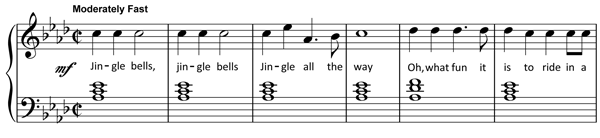
\includegraphics[width=\textwidth]{jingle-bells-sheet-music-piano.png}
\makeatletter
\let\@currsize\normalsize
\caption{Jingle bells melody sheet music representation	}
\label{fig:figure}
\end{figure}

Parsing digitized sheet music is an extremely challenging task. It requires a solid understanding on Computer Vision and even the state of the art software in existence today cant handle all scores (especially a poorly digitized formats). Given the amount of domain knowledge required, Modulo7 uses a third party library (insert TPL here). 

\subsection{Music XML format}
\noindent Music XML format is a standard open format for exchanging digital sheet music. A music XML format is unusual as its a format that is easy to parse for computers and easy for humans to understand it. MusicXML formats are heavily used by music notation applications. Music XML format is a symbolic format and can be considered a modernization of the Sheet music format. Its disadvantage however is unlike sheet music, a performer cant read the piece and play it on the spot directly. \\
Just like Western Sheet music and midi, music XML is a symbolic format as well. Music XML is also a transcription format which specifies how a score should be played. 

\subsection{MP3 format}
\noindent For the sake of completeness, Modulo7 also supports an audio format called mp3. Its an audio encoding format

